\documentclass{standalone}

\usepackage{comment}
\usepackage{xcolor}
\usepackage{tikz}
\usetikzlibrary{fit, matrix}
\usetikzlibrary{backgrounds}

\colorlet{rulecolor}{red!15}
\colorlet{linkcolor}{red!50}
\colorlet{cellcolor}{red!50}
\colorlet{textcolor}{red!75}
\colorlet{arrowcolor}{red!75}

% tex.stackexchange.com/questions/18521
\tikzset{
	table/.style={
		,matrix of nodes
		,row sep		= -\pgflinewidth
		,column sep		= -\pgflinewidth
		,nodes			= {rectangle, text width = 2em, align = center}
		,text depth		= 1ex
		,text height	= 2.0ex
		% ,nodes in empty cells
	}
	% ,letters/.style	 = {rectangle, fill = blue!50!white}
	,e/.style		 = {fill = none, text = textcolor}
	,row 1/.style    = {font=\ttfamily, nodes = {fill = cellcolor, text depth = 0.4ex, text height=2ex}}
	,column 1/.style = {font=\ttfamily, nodes = {fill = cellcolor}}
}

% arara: pdflatex: { draft: yes }
% arara: pdflatex: { synctex: no }
% arara: latexmk:  { clean: partial }
\begin{document}

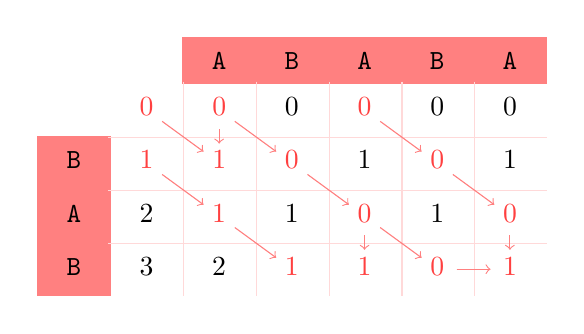
\begin{tikzpicture}

	% the matrix entries
	\matrix (mat) [table] {
	&   & A & B & A & B & A \\
	& |[e]|0 & |[e]|0 & 0 & |[e]|0 & 0 & 0 \\
	B   & |[e]|1 & |[e]|1 & |[e]|0 & 1 & |[e]|0 & 1 \\
	A   & 2 & |[e]|1 & 1 & |[e]|0 & 1 & |[e]|0 \\
	B   & 3 & 2 & |[e]|1 & |[e]|1 & |[e]|0 & |[e]|1 \\
	};

	% NOTE: the matrix rules
	% \begin{comment}
	\foreach \x in {2,...,4}{
		\draw[rulecolor]
		([xshift=-.5\pgflinewidth]mat-\x-2.south west) --
		([xshift=-.5\pgflinewidth]mat-\x-7.south east);
	}
	\foreach \x in {2,...,6}{
		\draw[rulecolor]
		([yshift=.5\pgflinewidth]mat-2-\x.north east) --
		([yshift=.5\pgflinewidth]mat-5-\x.south east);
	}
	% \end{comment}

	% the arrows
	\begin{scope}[shorten >=7pt,shorten <= 7pt]
		\filldraw[linkcolor, ->]  (mat-2-3.center) -- (mat-3-3.center);

		\filldraw[linkcolor, ->]  (mat-2-2.center) -- (mat-3-3.center);

		\filldraw[linkcolor, ->]  (mat-3-2.center) -- (mat-4-3.center);
		\filldraw[linkcolor, ->] (mat-4-3.center) -- (mat-5-4.center);

		\filldraw[linkcolor, ->]  (mat-2-3.center) -- (mat-3-4.center);
		\filldraw[linkcolor, ->]  (mat-3-4.center) -- (mat-4-5.center);
		\filldraw[linkcolor, ->]  (mat-4-5.center) -- (mat-5-6.center);
		\filldraw[linkcolor, ->]  (mat-4-5.center) -- (mat-5-5.center);

		\filldraw[linkcolor, ->]  (mat-2-5.center) -- (mat-3-6.center);
		\filldraw[linkcolor, ->]  (mat-3-6.center) -- (mat-4-7.center);
		\filldraw[linkcolor, ->]  (mat-4-7.center) -- (mat-5-7.center);

		\filldraw[linkcolor, ->]  (mat-5-6.center) -- (mat-5-7.center);
	\end{scope}
\end{tikzpicture}

\end{document}
